% !TEX TS-program = pdflatex
% !TEX encoding = UTF-8 Unicode

% This file is a template using the "beamer" package to create slides for a talk or presentation
% - Giving a talk on some subject.
% - The talk is between 15min and 45min long.
% - Style is ornate.

% MODIFIED by Jonathan Kew, 2008-07-06
% The header comments and encoding in this file were modified for inclusion with TeXworks.
% The content is otherwise unchanged from the original distributed with the beamer package.

\documentclass{beamer}


% Copyright 2004 by Till Tantau <tantau@users.sourceforge.net>.
%
% In principle, this file can be redistributed and/or modified under
% the terms of the GNU Public License, version 2.
%
% However, this file is supposed to be a template to be modified
% for your own needs. For this reason, if you use this file as a
% template and not specifically distribute it as part of a another
% package/program, I grant the extra permission to freely copy and
% modify this file as you see fit and even to delete this copyright
% notice. 

\usepackage{multimedia}
\usepackage{tipa}
\usepackage{natbib}
    \renewcommand{\bibsection}{\subsubsection*{\bibname } }
\usepackage{tikz}
\usetikzlibrary{arrows,shapes}

\newcommand{\tikzmark}[1]{\tikz[remember picture] \node[coordinate] (#1) {#1};}
\newcommand\mytextbullet{\leavevmode%
\usebeamertemplate{itemize item}}
\newcommand{\btVFill}{\vskip0pt plus 1filll}

\mode<presentation>
{
  \usetheme{Warsaw}
  % or ...

  \setbeamercovered{transparent}
  % or whatever (possibly just delete it)
}

\setbeamertemplate{footline}[frame number]
\usepackage[english]{babel}
% or whatever

\usepackage[utf8]{inputenc}
% or whatever

\usepackage{times}
\usepackage[T1]{fontenc}
% Or whatever. Note that the encoding and the font should match. If T1
% does not look nice, try deleting the line with the fontenc.


\title
{Attention and salience in lexically-guided perceptual learning}

\author
{Michael McAuliffe}
% - Use the \inst{?} command only if the authors have different
%   affiliation.

\institute
{}
% - Use the \inst command only if there are several affiliations.
% - Keep it simple, no one is interested in your street address.

\date
{PhD Defense}

\subject{Talks}
% This is only inserted into the PDF information catalog. Can be left
% out. 



% If you have a file called "university-logo-filename.xxx", where xxx
% is a graphic format that can be processed by latex or pdflatex,
% resp., then you can add a logo as follows:

% \pgfdeclareimage[height=0.5cm]{university-logo}{university-logo-filename}
% \logo{\pgfuseimage{university-logo}}





% If you wish to uncover everything in a step-wise fashion, uncomment
% the following command: 

%\beamerdefaultoverlayspecification{<+->}


\begin{document}

\begin{frame}
  \titlepage
\end{frame}

\section{Background}

\begin{frame}{Perceptual constancy}
\vfill
\begin{center}
Despite variation, listeners can interpret variable productions as a single word type
\vfill
\movie{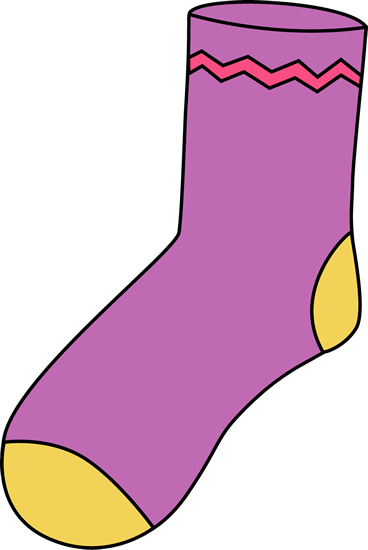
\includegraphics[width=0.1\textwidth]{pictures/sock}}{audio/variation.wav}

\end{center}
\btVFill

\begin{flushright}
\scriptsize
\citet{Shankweiler1977, Kuhl1979,Sumner2013}
\end{flushright}
\end{frame}

\subsection{Perceptual learning}

\begin{frame}{Perceptual learning}
\movie{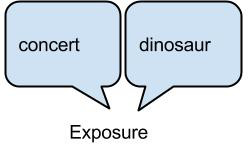
\includegraphics[width=0.45\textwidth]{pictures/exposure}}{audio/exposure.wav}
\hfill
\movie{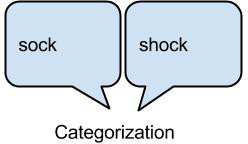
\includegraphics[width=0.45\textwidth]{pictures/categorization}}{audio/categorization.wav}

\end{frame}

\begin{frame}{Categorization}

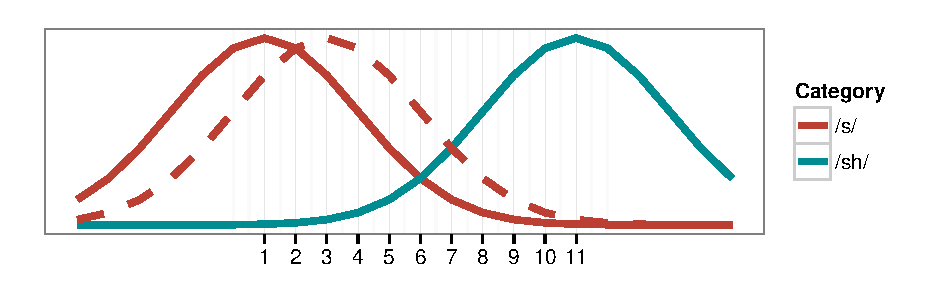
\includegraphics[width=0.905\textwidth]{graphs/dist}
\vfill
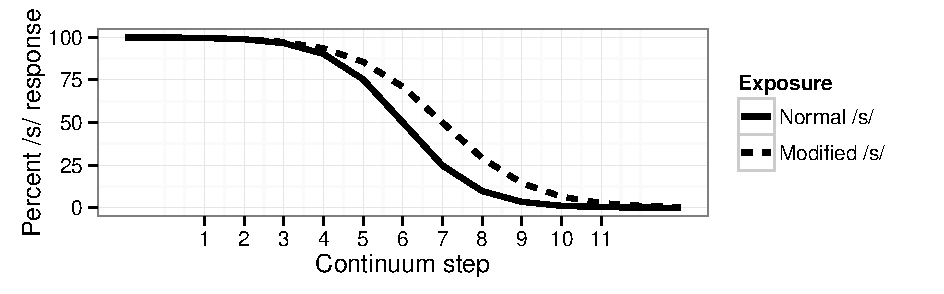
\includegraphics[width=1.0\textwidth]{graphs/class}

\end{frame}

\subsection{Sources of variation}

\begin{frame}{Sources of variation}

Example: /s/

\begin{minipage}[t]{0.45\textwidth}

\textbf{\textsc{Speaker}}

\begin{itemize}
\item Indexical
\begin{itemize}
\item Accent
\item Gender
\end{itemize}

\end{itemize}
\end{minipage}
\hfill
\begin{minipage}[t]{0.45\textwidth}
\textbf{\textsc{Listener}}

\begin{itemize}
\item Indexical
\begin{itemize}
\item Accent
\item Perceived accent
\item Perceived gender
\end{itemize}
\end{itemize}
\end{minipage}
\btVFill
\begin{flushright}
\scriptsize
\citet{Strand1996, Li2011, Kraljic2005}
\end{flushright}
\end{frame}

\begin{frame}{Sources of variation}

Example: /s/

\begin{minipage}[t]{0.45\textwidth}
\textbf{\textsc{Speaker}}

\begin{itemize}
\item Contextual
\begin{itemize}
\item Speaking rate
\item Coarticulation (/st\textturnr/)
\item Word position
\item Predictability
\end{itemize}

\end{itemize}
\end{minipage}
\hfill
\begin{minipage}[t]{0.45\textwidth}
\textbf{\textsc{Listener}}

\begin{itemize}
\item Contextual
\begin{itemize}
\item Speaking rate
\item Coarticulation (/st\textturnr/)
\item Word position
\item Predictability
\end{itemize}
\end{itemize}
\end{minipage}
\btVFill
\begin{flushright}
\scriptsize
\citet{Lieberman1963,Kraljic2008a,Clopper2008, Pitt2012}
\end{flushright}
\end{frame}

\begin{frame}{Sources of variation}

Example: /s/
\btVFill
\begin{minipage}[t]{0.45\textwidth}
\textbf{\textsc{Speaker}}

\begin{itemize}
\item Attention
\end{itemize}
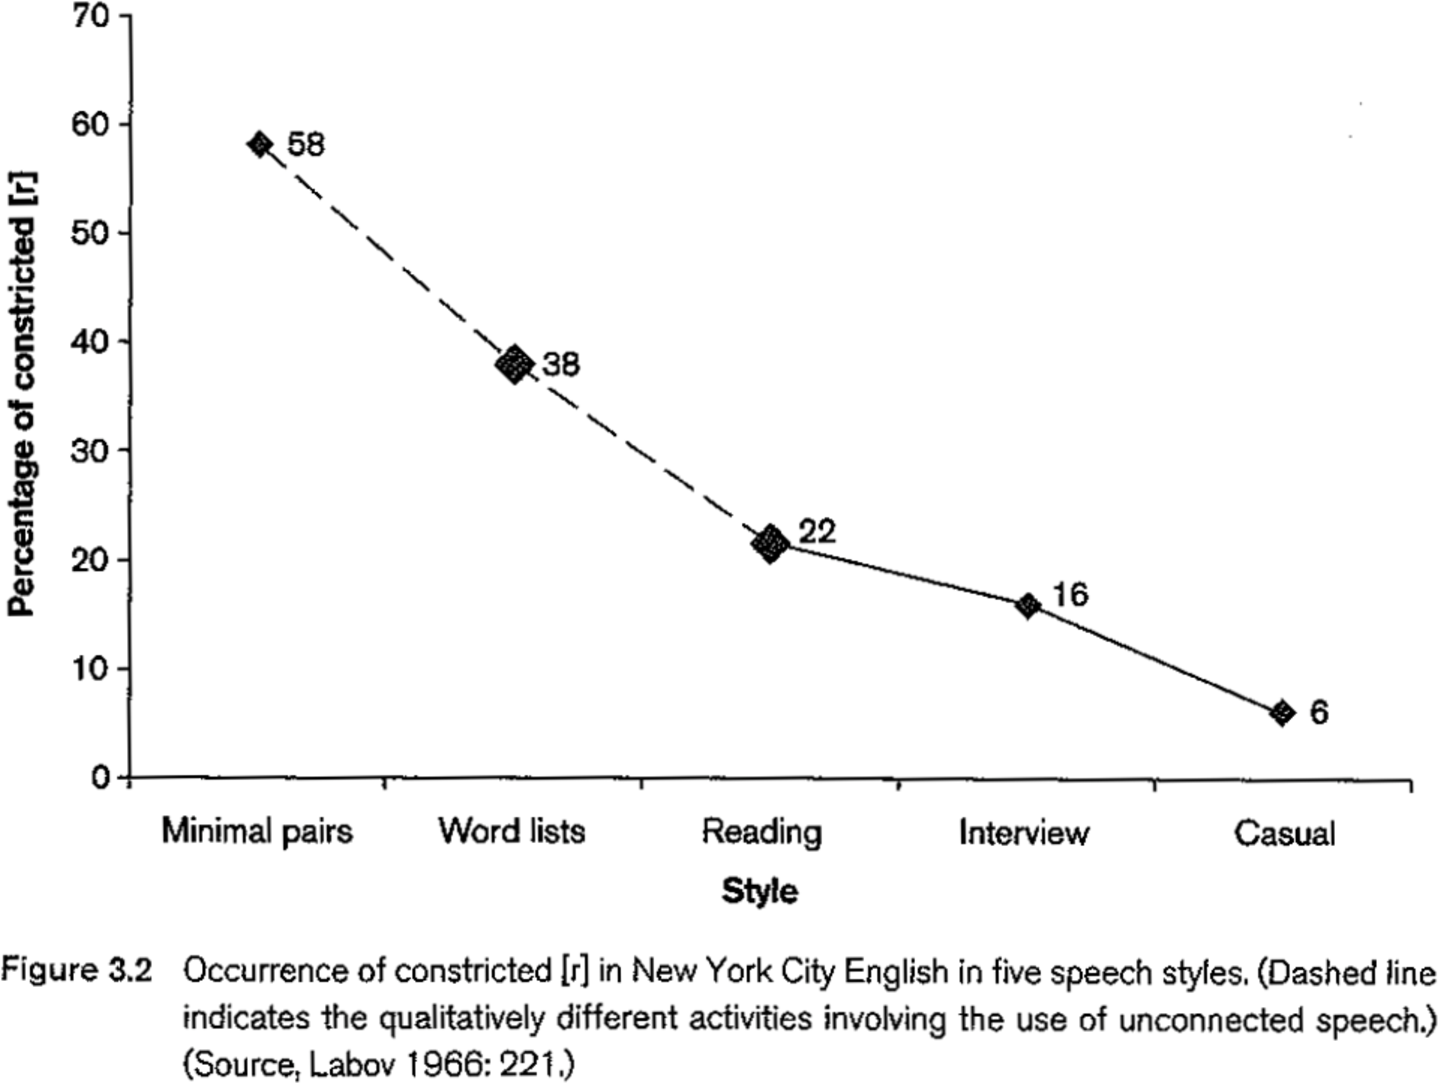
\includegraphics[width=1.3\textwidth]{pictures/Labov1997-mod}
\end{minipage}
\hfill
\begin{minipage}[t]{0.45\textwidth}
\textbf{\textsc{Listener}}

\begin{itemize}
\item Attention
\begin{itemize}
\item Comprehension
\item Perception
\end{itemize}
\end{itemize}
\end{minipage}
\btVFill
\begin{flushright}
\scriptsize
\citet{Labov1997, Pitt2012}
\end{flushright}
\end{frame}

\begin{frame}{Real world example}

\begin{itemize}
\item Students taught by a professor with non-native accent
\begin{itemize}
\item Some students will try to comprehend the lecture
\item Some students will get distracted by pronunciation
\item Some students will daydream
\item Do they all perceptually learn?
\end{itemize}
\end{itemize}

\end{frame}

\begin{frame}{Research question}

\vfill
How do changes to a listener's attention in exposure affect perceptual learning in future categorization?
\vfill

\end{frame}

\begin{frame}{Interaction of variation}

Example: /s/
\btVFill
\begin{minipage}[t]{0.45\textwidth}
Speaker

\begin{itemize}
\item Contextual
\begin{itemize}
\item Speaking rate
\item Coarticulation (/st\textturnr/)
\item \textbf{Word position} \tikzmark{n1} 
\item \textbf{Predictability} \tikzmark{n2} 
\end{itemize}
\item Attention
\end{itemize}
\end{minipage}
\hfill
\begin{minipage}[t]{0.45\textwidth}
Listener

\begin{itemize}
\item Contextual
\begin{itemize}
\item Speaking rate
\item Coarticulation (/st\textturnr/)
\item Word position
\item Predictability
\end{itemize}
\item[\tikzmark{t1} \mytextbullet] \textbf{Attention}
\begin{itemize}
\item Comprehension
\item Perception
\end{itemize}
\end{itemize}

\end{minipage}

\begin{tikzpicture}[remember picture,overlay]
        %\path[draw=magenta,thick,->]<3-> ([yshift=3mm]n1) to ++(0,3mm) to [out=0, in=0,distance=2.5in] (t1);
   \path[draw=magenta,thick,->] ([yshift=1.5mm]n1) --node[above,yshift=1.5mm] {$\scriptstyle Salience$} ([yshift=1.5mm]t1);
\end{tikzpicture}
\begin{tikzpicture}[remember picture,overlay]
        %\path[draw=magenta,thick,->]<3-> ([yshift=3mm]n1) to ++(0,3mm) to [out=0, in=0,distance=2.5in] (t1);
   \path[draw=magenta,thick,->] ([yshift=1.5mm]n2) -- ([yshift=1.5mm]t1);
\end{tikzpicture}
\btVFill
\end{frame}

\begin{frame}{Outline}
\tableofcontents
\end{frame}


\subsection{Attentional sets}

\begin{frame}{Attentional sets}

Strategies to parse our perceptual experience

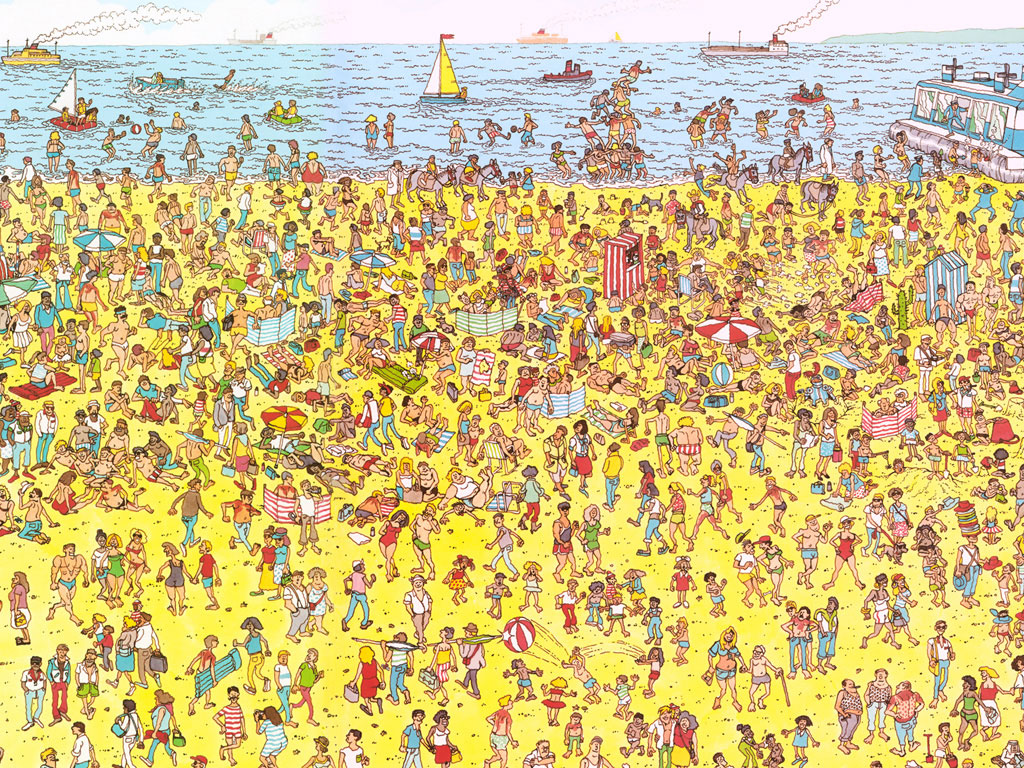
\includegraphics[width=0.9\textwidth]{pictures/waldo}

\end{frame}

\begin{frame}{Attentional sets}

\textbf{Comprehension-oriented}
\begin{itemize}
\item Focus on comprehending meaning
\item Real world example:

\begin{itemize}
\item Students in lecture
\item Primary focus is comprehending the professor (we hope)
\end{itemize}

\end{itemize}
\btVFill
\begin{flushright}
\scriptsize
\citet{Pitt2012}
\end{flushright}

\end{frame}

\begin{frame}{Attentional sets}

\textbf{Perception-oriented}
\begin{itemize}
\item Focus on perceiving a specific pronunciation
\item Real world example:
\begin{itemize}
\item Students in lecture
\item Professor with a non-native accent
\item Primary focus might shift from comprehension
\end{itemize}
\end{itemize}
\btVFill
\begin{flushright}
\scriptsize
\citet{Pitt2012}
\end{flushright}
\end{frame}

\begin{frame}{Attentional sets in perceptual learning}

\begin{itemize}
\item Comprehension-oriented tasks
\begin{itemize}
\item Lexical decision
\item Sentence transcription
\end{itemize}
\item Perception-oriented tasks
\begin{itemize}
\item Psychophysical perceptual learning
\item Audio-visual lipreading (nonwords)
\end{itemize}
\end{itemize}

\btVFill
\begin{flushright}
\scriptsize
\citet{Ahissar1993,Norris2003,Vroomen2007, Bradlow2008,Reinisch2014}
\end{flushright}

\end{frame}

\begin{frame}{Generalization in perceptual learning}

 Comprehension-oriented tasks generalize
\begin{itemize}
\item New words or nonwords
\item (Sometimes) new voices
\end{itemize}
Perception-oriented tasks do not generalize as readily
\begin{itemize}
\item Exposure specificity
\end{itemize}
\btVFill
\begin{flushright}
\scriptsize
\citet{Ahissar1993, Norris2003, Kraljic2005, Bradlow2008, Pitt2012, Reinisch2013}
\end{flushright}

\end{frame}


\begin{frame}{Hypothesis}
\vfill
Comprehension-oriented attentional sets allow for greater generalization than perception-oriented attentional sets.
\vfill
\end{frame}

\begin{frame}{Experimental paradigm}

Comprehension-oriented tasks
\begin{itemize}
\item Lexical decision
\item Word identification in sentences
\end{itemize}

Manipulations to promote perception-oriented attentional sets
\begin{itemize}
\item Instructions
\item Salience
\begin{itemize}
\item Unpredictability or low expectations
\item Increase the likelihood of listeners noticing modification
\item Assumption: similar to increasing the number of /s/ trials relative to filler trials

\end{itemize}

\end{itemize}

\end{frame}

\begin{frame}{Explicit instructions}
\btVFill
\begin{itemize}
\item ``This speaker's `s' sounds are ambiguous''
\item ``Please listen carefully to ensure you make the correct choice''
\item Promote perception-oriented attentional set
\end{itemize}

\btVFill
\begin{flushright}
\scriptsize
\citet{Pitt2012}
\end{flushright}
\end{frame}

\begin{frame}{Salience - Word position}

\begin{itemize}
\item Listeners are more tolerant of variation later in the word
\item Word-initial modified /s/ should be more salient
\item Examples
\begin{itemize}
\item Word-initial: \emph{submarine}
\item Word-medial: \emph{whistle}
\end{itemize}
\end{itemize}
\btVFill
\begin{flushright}
\scriptsize
\citet{Pitt2012}
\end{flushright}
\end{frame}

\begin{frame}{Salience - Category typicality}

\begin{itemize}
\item Productions farther from the mean of a category are more salient
\end{itemize}

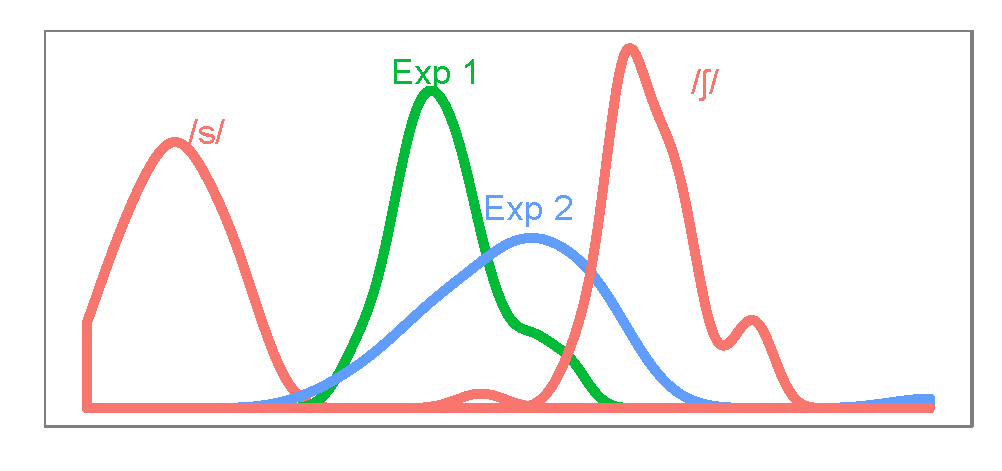
\includegraphics[width=1.0\textwidth]{graphs/salience}
\end{frame}

\section{Experiments 1 and 2}

\subsection{Set up}

\begin{frame}{Experiments 1 and 2}

Experiment 1
\begin{itemize}
\item Lexical decision exposure task
\item 94 native English participants
\item Across subject factors
\begin{itemize}
\item Instructions
\item Position of modified /s/ in words (Word-initial vs word-medial)
\end{itemize}
\item 50\% word response rate in a pre-test (n = 20)
\end{itemize}
Experiment 2
\begin{itemize}
\item Same design and materials as Experiment 1
\item 96 native English participants
\item 30\% word reponse rate in the pre-test (more atypical /s/)
\end{itemize}
\end{frame}

\begin{frame}{Sample trials}
Exposure
\begin{itemize}
\item Hear: whistle (\movie{Experiment 1}{audio/whistle_exp1.wav}) (\movie{Experiment 2}{audio/whistle_exp2.wav})
\item Hear: submarine (\movie{Experiment 1}{audio/submarine_exp1.wav}) (\movie{Experiment 2}{audio/submarine_exp2.wav})
\item Word or nonword?
\end{itemize}
\textbf{Categorization}
\begin{itemize}
\item Hear: sock-shock (\movie{continuum}{audio/categorization.wav}), sin-shin, sack-shack, sigh-shy
\item Sock or shock? Sin or shin? etc.
\end{itemize}
\end{frame}

\begin{frame}{Experiment 1 and 2 predictions}

Possible categorization outcomes:
\begin{itemize}
\item Equal perceptual learning effects across all conditions
\item Less perceptual learning when perception-oriented attentional sets are promoted
\begin{itemize}
\item Primary hypothesis
\end{itemize}
\item Perceptual learning effects stronger in Word-initial exposure condition
\begin{itemize}
\item More similar to categorization items
\end{itemize}
\end{itemize}
\end{frame}

\subsection{Results}

\begin{frame}{Experiment 1 - Word-initial exposure}

\begin{minipage}{0.4\textwidth}
\textbf{Ambiguous /s/}
\begin{itemize}
\item 50\% between /s/ and /\textesh/
\end{itemize}

\textbf{Attention}
\begin{itemize}
\item No /s/-oriented instructions
\item Told /s/ would be ambiguous
\end{itemize}

\textbf{Position of /s/}
\begin{itemize}
\item \emph{Word initial}
\item Word medial
\end{itemize}
\end{minipage}
\hfill
\begin{minipage}{0.53\textwidth}
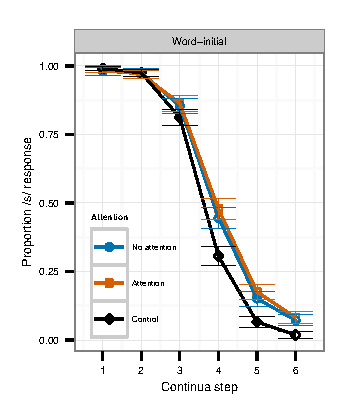
\includegraphics[width=1.0\textwidth]{graphs/exp1_categresults_present2-initial}
\end{minipage}

\end{frame}

\begin{frame}{Experiment 1 - Word-medial exposure}

\begin{minipage}{0.4\textwidth}
\textbf{Ambiguous /s/}
\begin{itemize}
\item 50\% between /s/ and /\textesh/
\end{itemize}

\textbf{Attention}
\begin{itemize}
\item No /s/-oriented instructions
\item Told /s/ would be ambiguous
\end{itemize}

\textbf{Position of /s/}
\begin{itemize}
\item Word initial
\item \emph{Word medial}
\end{itemize}
\end{minipage}
\hfill
\begin{minipage}{0.53\textwidth}
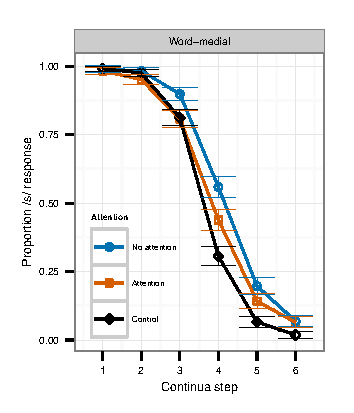
\includegraphics[width=1.0\textwidth]{graphs/exp1_categresults_present2-final}
\end{minipage}

\end{frame}

\begin{frame}{Experiment 2 - Word-initial exposure}

\begin{minipage}{0.4\textwidth}
\textbf{Ambiguous /s/}
\begin{itemize}
\item More like /\textesh/ than /s/
\end{itemize}

\textbf{Attention}
\begin{itemize}
\item No /s/-oriented instructions
\item Told /s/ would be ambiguous
\end{itemize}

\textbf{Position of /s/}
\begin{itemize}
\item \emph{Word initial}
\item Word medial
\end{itemize}
\end{minipage}
\hfill
\begin{minipage}{0.53\textwidth}
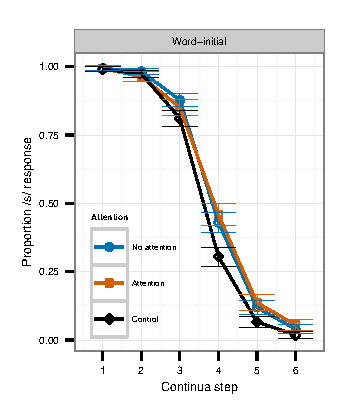
\includegraphics[width=1.0\textwidth]{graphs/exp2_categresults_present2-initial}
\end{minipage}

\end{frame}

\begin{frame}{Experiment 2 - Word-medial exposure}

\begin{minipage}{0.4\textwidth}
\textbf{Ambiguous /s/}
\begin{itemize}
\item More like /\textesh/ than /s/
\end{itemize}

\textbf{Attention}
\begin{itemize}
\item No /s/-oriented instructions
\item Told /s/ would be ambiguous
\end{itemize}

\textbf{Position of /s/}
\begin{itemize}
\item Word initial
\item \emph{Word medial}
\end{itemize}
\end{minipage}
\hfill
\begin{minipage}{0.53\textwidth}
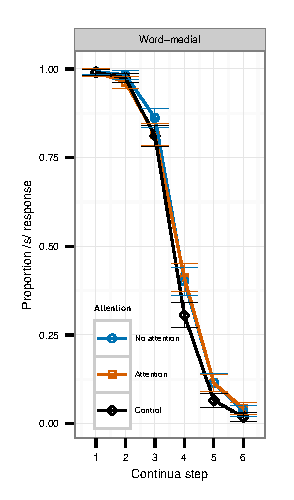
\includegraphics[width=1.0\textwidth]{graphs/exp2_categresults_present2-final}
\end{minipage}

\end{frame}

\subsection{Summary}

\begin{frame}{Summary}

\begin{itemize}
\item Results align with attentional sets
\item Conditions promoting a perception-oriented attentional set
\begin{itemize}
\item Had smaller perceptual learning effects
\item Still showed perceptual learning
\item Did not differ from one another
\end{itemize}
\item Fine-grained similarity did not appear to play a role
\begin{itemize}
\item Word-medial exposure had the largest effect

\end{itemize}
\end{itemize}

\end{frame}

\begin{frame}{Further promoting comprehension}

\begin{itemize}

\item Lexical decision is comprehension-oriented
\begin{itemize}
\item Word recognition
\end{itemize}
\item Experiment 3 uses words in sentences
\begin{itemize}
\item Attempt to further promote comprehension
\end{itemize}
\end{itemize}

\end{frame}

\section{Experiment 3}

\subsection{Set up}

\begin{frame}{Exposure task}
\begin{itemize}
\item Predictable: The traffic cop alerted the driver by blowing her whistle (\movie{Audio}{audio/P_whistle.wav}) 
\item Unpredictable: The boy ran away when he heard the whistle(\movie{Audio}{audio/U_whistle.wav})
\end{itemize}
\begin{minipage}[t]{0.45\textwidth}
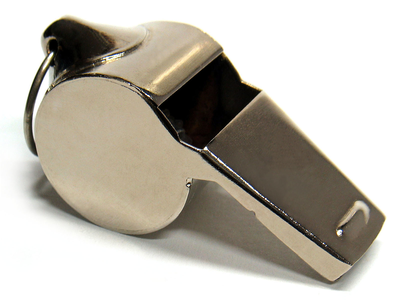
\includegraphics[width=1.0\textwidth]{pictures/whistle}
\end{minipage}
\hfill
\begin{minipage}[t]{0.45\textwidth}
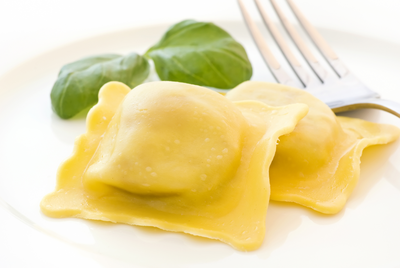
\includegraphics[width=1.0\textwidth]{pictures/ravioli}
\end{minipage}
\end{frame}

\begin{frame}{Salience - Semantic predictability}

\begin{itemize}
\item Listeners are more tolerant of acoustic reduction or noise in predictable sentences
\item Modified /s/ should be more salient in unpredictable words
\item Examples
\begin{itemize}
\item Predictable: The cow gave birth to the calf.
\item Unpredictable: She is glad Jane called about the calf.
\end{itemize}
\end{itemize}
\btVFill
\begin{flushright}
\scriptsize
\citet{Lieberman1963, Kalikow1977, Scarborough2010}
\end{flushright}
\end{frame}

\begin{frame}{Experiment 3}

\begin{itemize}
\item 98 native English participants
\item Cross-modal word identification
\begin{itemize}
\item Auditory sentences
\item Identification of picture corresponding to final word in sentence
\item Same word-medial modified /s/ stimuli (Experiment 1)
\item Final targets were predictable or unpredictable (pre-test)
\end{itemize}
\item Across subjects
\begin{itemize}
\item Instructions (identical to Experiments 1 and 2)
\item Modified /s/ only in predictable or unpredictable words
\end{itemize}
\item \textbf{Same categorization as Experiment 1 and 2}
\end{itemize}

\end{frame}

\begin{frame}{Experiment 3 categorization predictions}

Within sentences:
\begin{itemize}
\item Equal perceptual learning 
\item Bigger perceptual learning effect in predictable exposure
\begin{itemize}
\item Less salient modification
\end{itemize}
\item Smaller perceptual learning effect in predictable exposure
\begin{itemize}
\item Attribution of variation to predictability
\end{itemize}
\end{itemize}
\end{frame}

\begin{frame}{Experiment 3 categorization predictions}

Words in isolation vs in sentences
\begin{itemize}
\item Equal perceptual learning
\item Bigger perceptual learning effect in sentences
\begin{itemize}
\item Comprehension of sentences rather than words
\end{itemize}
\item Smaller perceptual learning effect in sentences
\begin{itemize}
\item Less speaker attention in read sentences
\end{itemize}
\end{itemize}
\end{frame}

\subsection{Results}

\begin{frame}{Experiment 3 - Unpredictable exposure}

\begin{minipage}{0.4\textwidth}
\begin{itemize}
\item \textbf{Ambiguous /s/}
\begin{itemize}
\item Halfway between /s/ and /\textesh/
\item In sentences
\end{itemize}

\item \textbf{Attention}
\begin{itemize}
\item No /s/-oriented instructions
\item Told /s/ would be ambiguous
\end{itemize}

\item \textbf{Predictability of final /s/ words}
\begin{itemize}
\item \emph{Unpredictable}
\item Predictable
\end{itemize}
\end{itemize}
\end{minipage}
\hfill
\begin{minipage}{0.53\textwidth}
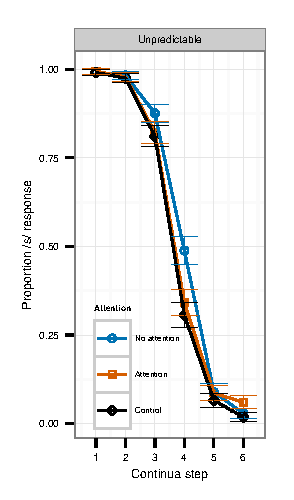
\includegraphics[width=1.0\textwidth]{graphs/exp3_categresults_present2-unpredictable}
\end{minipage}

\end{frame}

\begin{frame}{Experiment 3 - Predictable exposure}

\begin{minipage}{0.4\textwidth}
\begin{itemize}
\item \textbf{Ambiguous /s/}
\begin{itemize}
\item Halfway between /s/ and /\textesh/
\item In sentences
\end{itemize}

\item \textbf{Attention}
\begin{itemize}
\item No /s/-oriented instructions
\item Told /s/ would be ambiguous
\end{itemize}

\item \textbf{Predictability of final /s/ words}
\begin{itemize}
\item Unpredictable
\item \emph{Predictable}
\end{itemize}
\end{itemize}
\end{minipage}
\hfill
\begin{minipage}{0.53\textwidth}
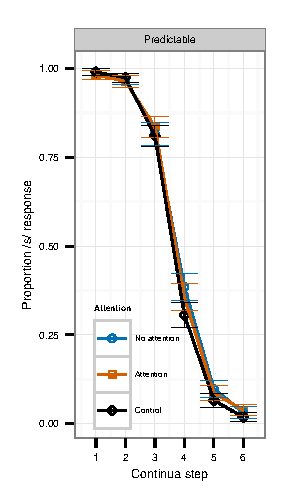
\includegraphics[width=1.0\textwidth]{graphs/exp3_categresults_present2-predictable}
\end{minipage}

\end{frame}

\begin{frame}{Isolation vs Sentences}

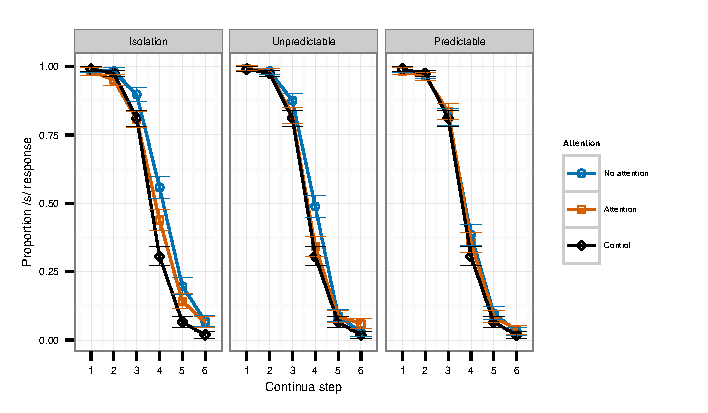
\includegraphics{graphs/exp23_categresults_present}
\end{frame}

\subsection{Summary}

\begin{frame}{Summary}

\begin{itemize}
\item Unpredictable exposure showed a similar pattern to words in isolation
\item Predictable exposure showed no perceptual learning effect
\begin{itemize}
\item Similar to studies using a coarticulation context (/st\textturnr/)
\item Predictable words are typically shorter and less clear
\item Listeners compensate for this predictability
\item Mean durations: Predictable words (0.53 s, SD = 0.06 s), Unpredictable words (0.53 s, SD = 0.07 s)
\end{itemize}
\btVFill
\begin{flushright}
\scriptsize
\citet{Clopper2008, Scarborough2010,Kraljic2008a}
\end{flushright}
\end{itemize}

\end{frame}

\section{Discussion}

\begin{frame}{Discussion}

\begin{itemize}
\item Attentional sets affected perceptual learning
\begin{itemize}
\item Conditions that did not promote perception-oriented attentional sets showed larger effects
\end{itemize}
\item Predictability was not an effective attentional set manipulation
\begin{itemize}
\item Instead, allowed for attribution of the modified category to predictability
\end{itemize}
\end{itemize}

\end{frame}

\begin{frame}{Implications for theoretical models}

\begin{itemize}
\item Supports hierarchical representations
\item Attention to episodic representations or specific pronunciations inhibits learning in abstract categories
\item Attention as a gain mechanism is not supported
\begin{itemize}
\item Perception-oriented attentional sets would have larger effects
\item Valency of attention may play a role
\end{itemize}
\end{itemize}
\end{frame}

\begin{frame}{Implications - Dialects}

\begin{itemize}
\item Perceptual learning of salient dialectal features may be inhibited
\begin{itemize}
\item New Zealand/Australian English: \emph{fish and chips}
\item New Zealand/North American English: \emph{Bret} vs \emph{Brit}
\end{itemize}
\end{itemize}


\end{frame}

\begin{frame}{Implications - Non-native accents}
\begin{itemize}
\item Non-native listener / native speaker
\begin{itemize}
\item Perception-oriented attentional set may be the default
\end{itemize}

\item Native listener / non-native speaker
\begin{itemize}
\item Perceptual learning inhibited when attending to pronunciation
\end{itemize}
\end{itemize}
Real world example:
\begin{itemize}
\item Students attending to the professor's message rather than pronunciation should perceptually adapt more
\begin{itemize}
\item Timecourse of perceptual learning?
\item Size of perceptual learning?
\end{itemize}
\end{itemize}

\end{frame}

\begin{frame}{Acknowledgements}
\centering
\vfill
Thank you to all those involved drafting and creating these experiments, particularly Molly Babel, Eric Vatikiotis-Bateson, Carla Hudson Kam, Graham Haber, Jamie Russell, Jobie Hui and Michelle Chan!
\vfill
Feedback from various 530 helped tremendously in shaping the ideas and experiments in this thesis.
\vfill
Thank you all for your attention!
\vfill
\end{frame}

\begin{frame}[allowframebreaks]{References}%in case more than 1 slide needed
    \footnotesize
\bibliographystyle{apalike}
\bibliography{biblio}
\end{frame}


\begin{frame}{Experiment 1 - Acoustic analysis}
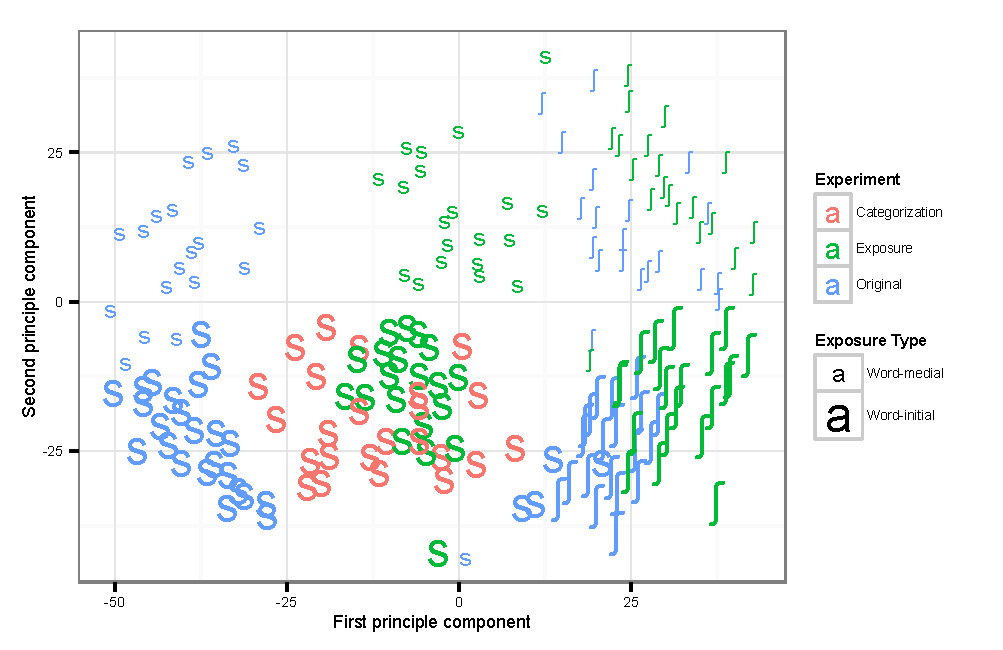
\includegraphics[width=1.0\textwidth]{graphs/exp1_mds}
\end{frame}

\begin{frame}{Experiment 1 - Exposure ACC}
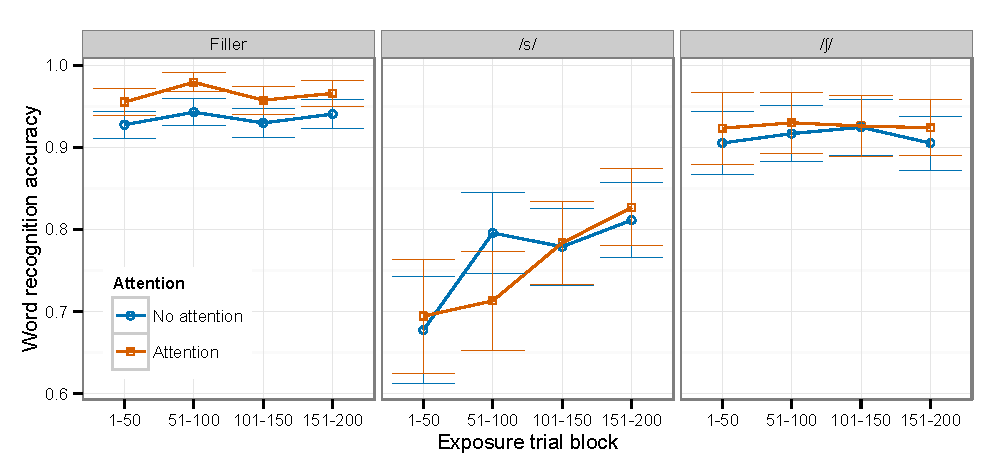
\includegraphics[width=1.0\textwidth]{graphs/exp1_expacc}
\end{frame}

\begin{frame}{Experiment 1 - Exposure RT}
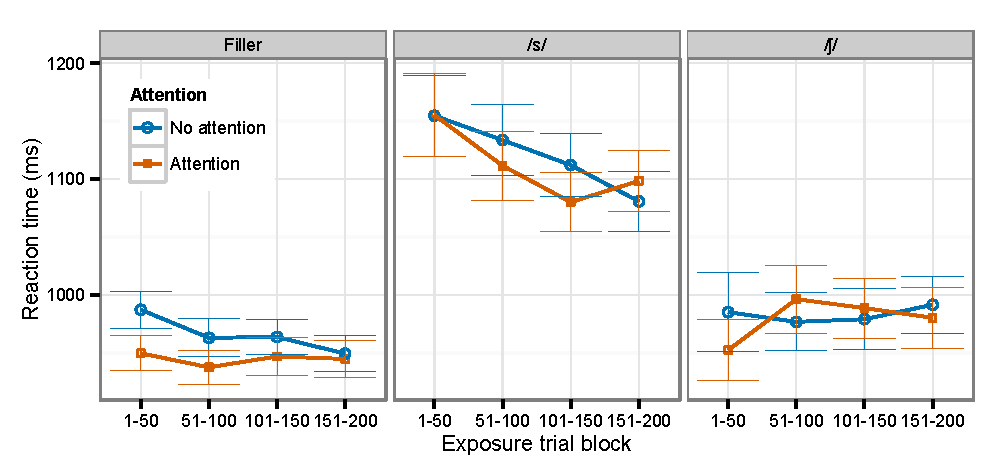
\includegraphics[width=1.0\textwidth]{graphs/exp1_exprt}
\end{frame}

\begin{frame}{Experiment 2 - Acoustic analysis}
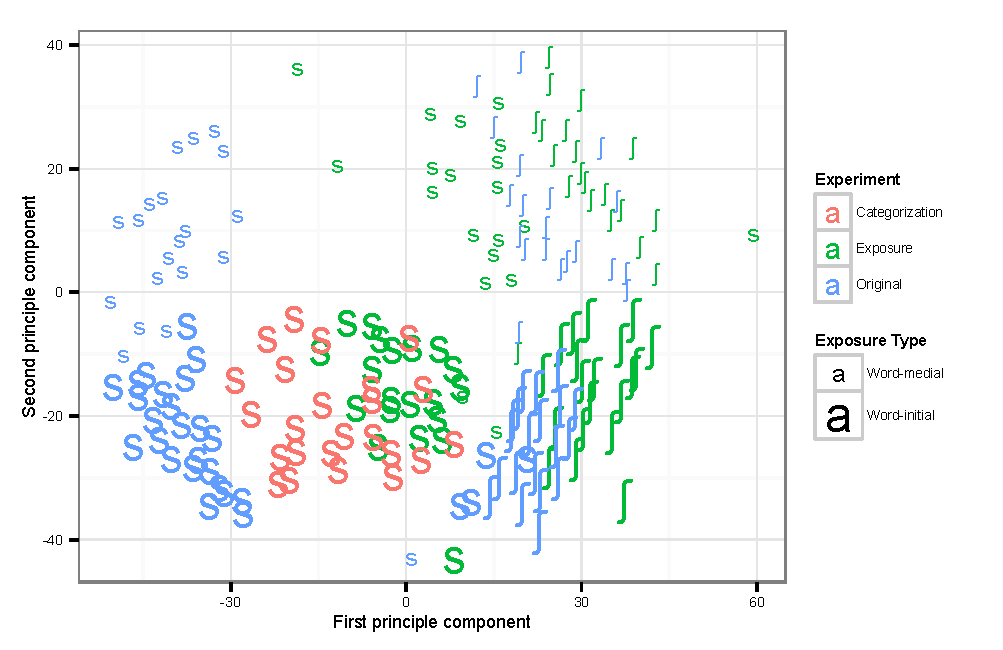
\includegraphics[width=1.0\textwidth]{graphs/exp2_mds}
\end{frame}


\begin{frame}{Experiment 2 - Exposure ACC}
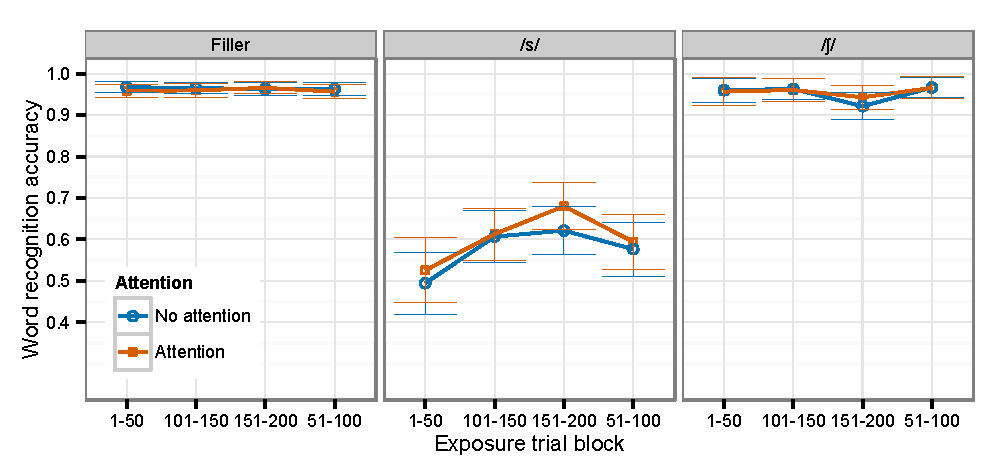
\includegraphics[width=1.0\textwidth]{graphs/exp2_expacc}
\end{frame}

\begin{frame}{Experiment 2 - Exposure RT}
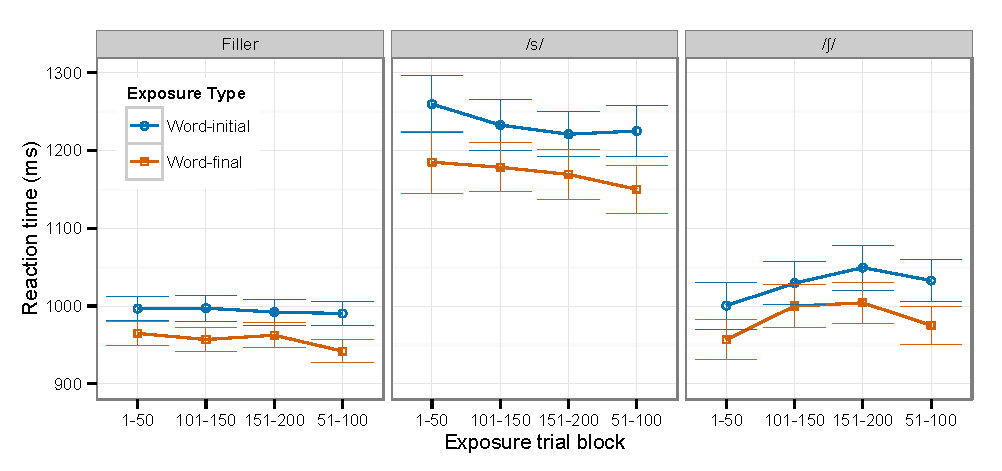
\includegraphics[width=1.0\textwidth]{graphs/exp2_exprt}
\end{frame}



\begin{frame}{Experiments 1 and 2 - Cross-over and word responses}
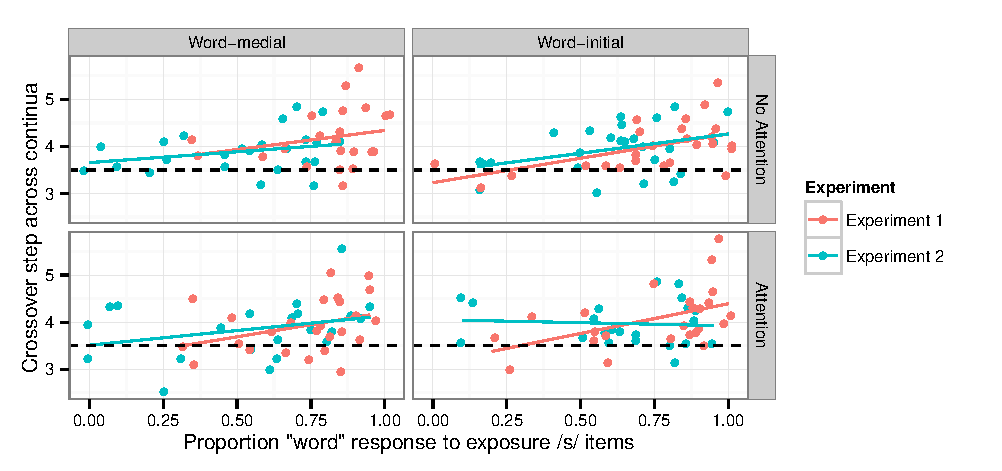
\includegraphics[width=1.0\textwidth]{graphs/exp12_xoverwordresp}
\end{frame}

\begin{frame}{Experiment 3 - Acoustic analysis}
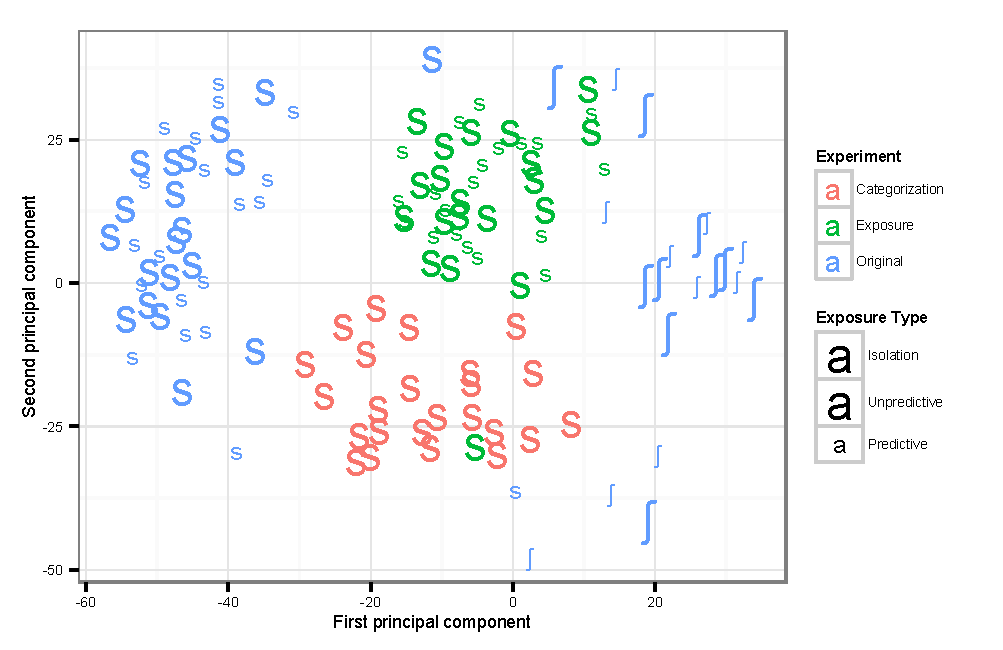
\includegraphics[width=1.0\textwidth]{graphs/exp3_mds}
\end{frame}

\begin{frame}{Experiment 3 - Exposure RT}
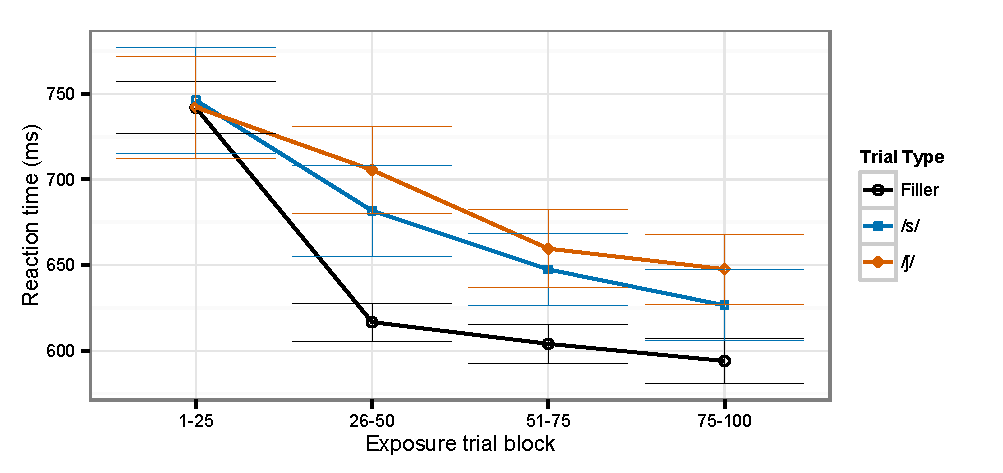
\includegraphics[width=1.0\textwidth]{graphs/exp3_exprt}
\end{frame}

\begin{frame}{Experiment 1 and 3 - Cross-over distribution}
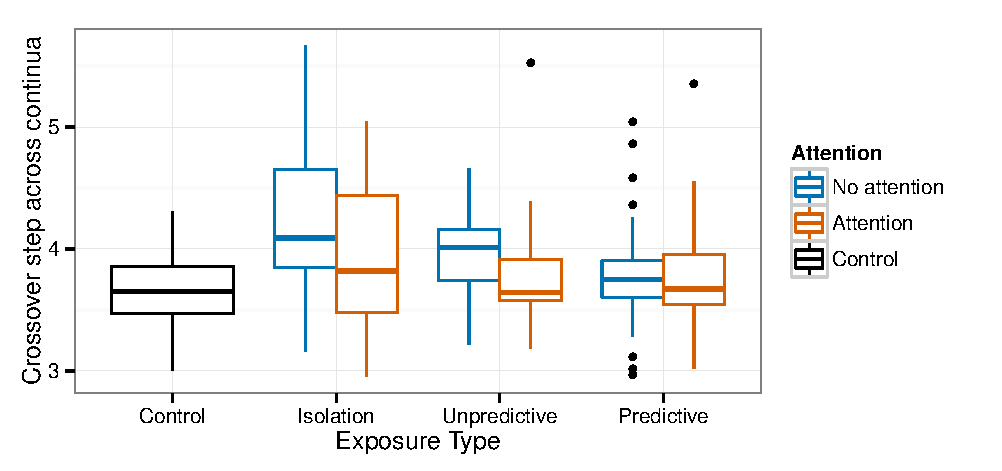
\includegraphics[width=1.0\textwidth]{graphs/exp13_xoverdist}
\end{frame}
\end{document}


